%\chapter{Numerical Examples}
\chapter{従来手法}

\section{問題設定}

本研究は静的な環境下で教示される物体移動動作から、被移動物体(以下、トラジェクタ)の目標位置の決定に関与する参照点とその位置関係を推定する手法について提案する。
そのため本研究では、ある地点に置いてある物体をある法則に従った他の地点に移動するという、初期状態と最終状態の対を動作と定義し、動作ごとに固有の法則を観点と呼ぶ。観点は参照点と、参照点に対する位置関係を表す変位の対と定義する。また任意の初期状態に対し、教示者の意図するトラジェクタの目標位置は一意に定まるものとする。即ち、例えばトラジェクタを物体の右に動かすという動作に関して、教示者は常にその物体から一定の距離だけ右の位置にトラジェクタを移動することを意識しているものとし、動作教示時に生じる誤差は教示精度に依るものであり、教示者の意図する目標位置自体の曖昧さに依るものではないとする。

\section{従来手法}

\subsection{参照点}

杉浦ら\cite{sugiura}の手法において、参照点は環境中の物体の位置、トラジェクタの初期位置(動作開始点)、画面中央としている。
トラジェクタの遷移には、大別すると以下の3種類が存在するとしている。

	\begin{enumerate}
		\item 初期状態に関わらず、トラジェクタの初期位置に対して一定の遷移を行う
		\item 初期状態に関わらず、空間上の特定の位置に遷移を行う
		\item 1つ以上の物体の位置や相対位置に応じて遷移先が変化する
	\end{enumerate}
これら3種類の違いについてFig.\ref{figure:2_moving_trajector}で示す。
%%%%%%%%%%%%%%%%%%%%%%%%%%%%%%%%%%%%%%%%%%%%%%%%%%%%%%%%%%%%%%%%%%%%%%%%%%%%%%%%%%%%%%%%%%%%%%%%%%%%%%%
	\begin{figure}[h]
%中央ぞろえ
		\begin{center}
			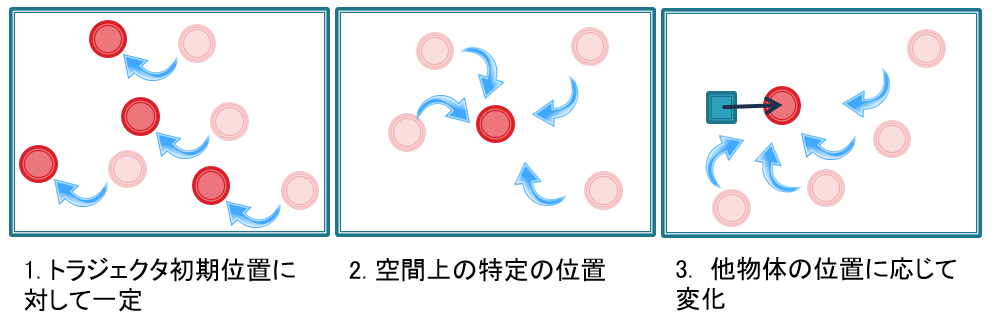
\includegraphics[width=14cm]{figure1.png} \\ %eXの基本として, \\ で緊急改行ができる。(今回の場合や行列などを除き、あまり使わない)
			\caption{トラジェクタ遷移の違い}
			\label{figure:2_moving_trajector}
		\end{center}
	\end{figure}
%%%%%%%%%%%%%%%%%%%%%%%%%%%%%%%%%%%%%%%%%%%%%%%%%%%%%%%%%%%%%%%%%%%%%%%%%%%%%%%%%%%%%%%%%%%%%%%%%%%%%%%
1はトラジェクタの初期位置を、2は画面中央を参照点に含めることで、3の特殊な事例として実現できるため、全ての物体移動動作は参照点との相対位置を考慮した目標位置を持つとしている。

\subsection{変位}

特定の参照点に対し、動作はさらに以下の2種類が存在するとしている。

	\begin{enumerate}
		\item 参照点を原点とし、常に一定の相対位置に遷移する
		\item 参照点を原点とし、トラジェクタの初期位置に応じて遷移先が変化する
	\end{enumerate}
これら2種類の違いについてFig.\ref{figure:2_difference_displacement}で示す。
%%%%%%%%%%%%%%%%%%%%%%%%%%%%%%%%%%%%%%%%%%%%%%%%%%%%%%%%%%%%%%%%%%%%%%%%%%%%%%%%%%%%%%%%%%%%%%%%%%%%%%%
	\begin{figure}[t]
%中央ぞろえ
		\begin{center}
			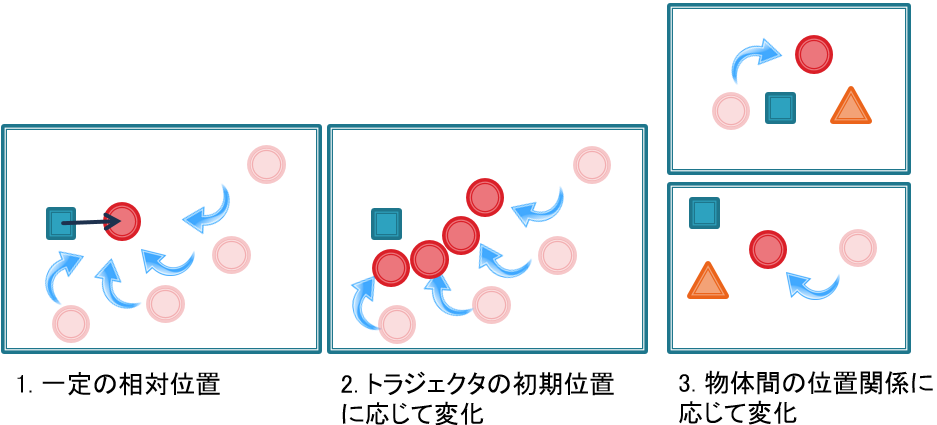
\includegraphics[width=14cm]{figure2.png} \\ %Teの基本として, \\ で緊急改行ができる。(今回の場合や行列などを除き、あまり使わない)
			\caption{参照点に対する遷移の違い}
			\label{figure:2_difference_displacement}
		\end{center}
	\end{figure}
%%%%%%%%%%%%%%%%%%%%%%%%%%%%%%%%%%%%%%%%%%%%%%%%%%%%%%%%%%%%%%%%%%%%%%%%%%%%%%%%%%%%%%%%%%%%%%%%%%%%%%%
1は例えばトラジェクタを物体の右隣に動かすという動作などで、参照点である物体に関して常に相対位置が一定である。2はトラジェクタを物体に近づけるという動作などで、これは参照点となる物体とトラジェクタの初期位置の位置関係によって、参照点からの目標位置の相対位置が変化する。従来手法ではこれらを判別する方法として、学習時に複数の座標軸系考慮している。例えば1の動作では、参照点を原点として画面に平行な座標系を考慮することで実現することができ、2の動作では、参照点を原点としてトラジェクタの初期位置に軸を向けた座標系を考慮することで実現することができる。

\subsection{学習、再現}

従来手法では教示動作が与えられたとき、以下の式を用いて尤度が最大となる参照点$\hat{m}$、座標系$\hat{k}$、モデルのパラメータ$\hat{λ}$を最尤推定により学習している。
\begin{equation}
	\label{equation:sugiura}
	(\hat{λ} , \hat{k} , \hat{m}) = \mathop{\arg\max}_{λ , k , m}\sum_{i=1}^{N}\log P(F(Y_{i} , k , m_{i}) ; λ)
\end{equation}
ここで、$Y_{i}$はトラジェクタの位置、速度、加速度の時系列データ、$m_{i}$は参照点、$F(Y , k , m)$は座標系$k$、参照点$m$としたときのトラジェクタの動作軌道、$P(F,λ)$は動作軌道$F$がパラメータ$λ$の確率モデルから生成される確率である。杉浦らの研究では動作軌道を再現することを目標の一つとしていたため、確率モデルに時系列データを扱える隠れマルコフモデルを使用している。動作再現は\ref{equation:sugiura}式の最尤推定によって推定されたパラメータ$λ$を持つ隠れマルコフモデルからトラジェクタ遷移情報の時系列を生成することで実現する。
この手法では参照点を各物体の位置、トラジェクタの動作開始点、画面中央に限定している。この手法では複数の物体間の位置関係を学習時に扱うことができず、椅子を等間隔に並べるなどの動作を適切に再現することができない。